%
% CHAPTER Versuch 2
%
\chapter{Spracherkennung}
Dieser Abschnitt befasst sich mit der eigentlichen Spracherkennung und greift auf die Ergebnisse der vorigen Teilaufgabe zurück.
\label{chap:FrequenzgangVonLautsprechern}
\section{Fragestellung, Messprinzip, Aufbau, Messmittel}
\label{chap:VERSUCH_2_FRAGESTELLUNG}
Für den Aufbau des Spracherkenners wird auf das in der Vorlesung behandelte Prinzip
des Prototypenklassifikators zurückgegriffen. \cite[S.24]{Franz2015i}
Gemäß dieser Mustererkennung wurde für die Wörter \textit{Hoch, Tief, Links, Rechts} jeweils ein Referenzspektrum gebildet. Diese Spektren werden in der Mustererkennung mit dem jeweiligen Eingabewort verglichen. Dieser Vergleich wird mit dem Verfahren der Kovarianz durchgeführt. Im Gegensatz zur Bestimmung der Ähnlichkeit mit Korrelation wird bei der Kovarianz zunächst bei jedem Signal der Mittelwert des selbigen abgezogen. Auf diese Weise können auch unterschiedlich große Signale, die den gleichen Signalverlauf haben als übereinstimmend erkannt werden. Praktisch wird dadurch die Möglichkeit gegeben ein Wort laut auszusprechen oder auch leise. Beide Male würde das Wort erkannt werden. Zum Vergleich der Signale findet der Korrelatioinskoeffizient nach Bravais-Pearson Einsatz, um die Spektren zu vergleichen.
Der Korrelationskoeffizient ergibt sich aus dem Quotienten der Kovarianz beider Signale und dem Produkt der einzelnen Standartabweichungen. Der Korrelatinskoeffizient nach Bravais-Pearson hat somit einen Wertebereich von -1.0 bis 1.0. Werte nahe bei 1.0 bedeuten eine hohe Ähnlichkeit. Handelt es sich bei dem Ergebnis um die Zahl null ist keine Ähnlichkeit vorhanden. Bekommt man als Resultat eine Zahl nahe an -1 ist diese als "Anti-Ähnlichkeit" zu deuten.\cite[S.27]{Franz2015i}
Da ein Mensch kein technisches System ist, ist nicht gewährleistet, dass ein eben ausgesprochenes Wort im nächsten Moment exakt gleich klingt wenn es nochmals ausgesprochen wird. Aufgrund dieser Tatsache wird das Referenzspektrum aus dem Mittel der Spektren von Fünf verschiedenen Aufnahmen gebildet. Für die Messung des Refereznspektrums muss darf der Sprecher nicht wechseln.
Sind die Referenzspektren erstellt kann nun nach der Vorgestellten Methode der Kovarianz ein Vergleich stattfinden. Das Signalpaar, dass den größten Korrelationskoeffizienten hat, welcher zusätzlich noch größer als 0.9 sein muss wird als übereinstimmend betrachtet. Die Zahl 0.9 wurde experimentell ermittelt.
Es wird also nicht einfach das Wort genommen, dass den größten Korrelationskoeffizienten hat. Würde man ein beliebiges Wort, für welches es kein Referenzspektrum gibt, in den Spracherkenner eingeben, wurde dieser sich für das Wort mit dem ähnlichsten Spektrum entscheiden, selbst wenn die Spektren sehr verschieden sind.
Zum Testen des Spracherkenners werden Zwei Testdatensätze mit jeweils Fünf Aufnahmen für jedes Wort, das der Spracherkenner beherrscht aufgenommen. Bei dem ersten Testdatensatz spricht der Sprecher, der auch in den Aufnahmen für das Referenzspektrum gesprochen hat.
Im zweiten Satz spricht ein anderer Sprecher. Es ergeben sich 40 Sprachaufnahmen, die automatisiert in den Spracherkenner geladen werden. Das Ergebnis wird untersucht, ob es dem Erwarteten entspricht, um so die Zuverlässigkeit des Spracherkenners zu testen.
Der Spracherkenner selbst bekommt diese Testaufnahmen im Zeitbereich und muss zuerst mit den aus dem ersten Aufgabenteil entwickelten Methoden eine Fourieranalyse durchführen. Diese Aufnahmen wurden bei der Aufnahme auch schon getriggert.
\newpage
\section{Messwerte}
\label{chap:VERSUCH_2_MESSWERTE}
\begin{figure}[H]
    \centering
    \begin{subfigure}[b]{0.49\textwidth}
        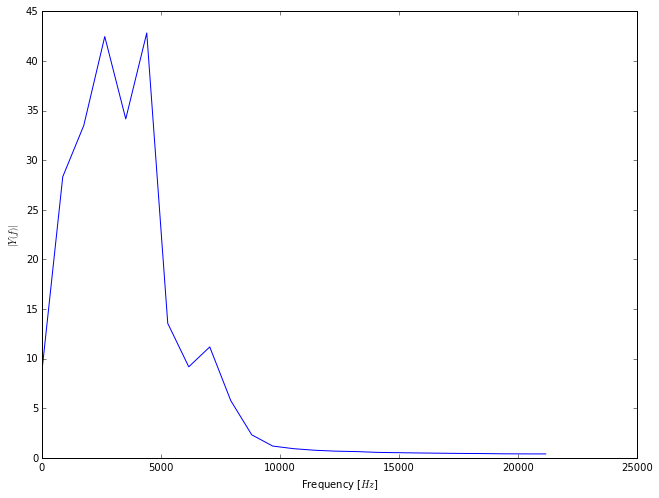
\includegraphics[width=\textwidth]{Hoch.png}
        \caption{Hoch}
        \label{fig:Hoch}
    \end{subfigure}
    ~ %add desired spacing between images, e. g. ~, \quad, \qquad, \hfill etc. 
      %(or a blank line to force the subfigure onto a new line)
    \begin{subfigure}[b]{0.49\textwidth}
        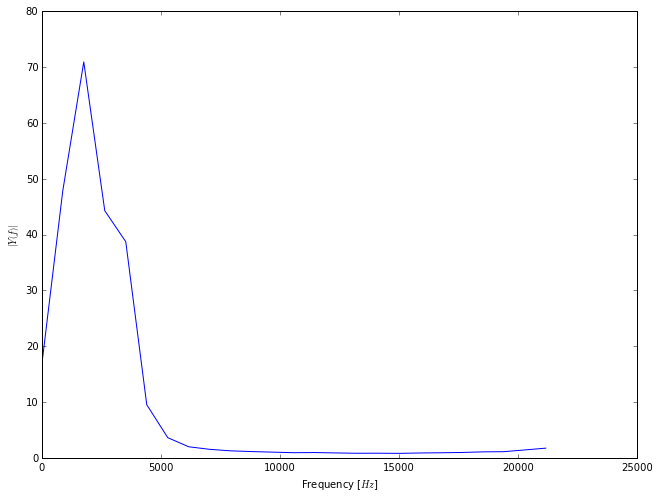
\includegraphics[width=\textwidth]{Tief.png}
        \caption{Tief}
        \label{fig:Tief}
    \end{subfigure}
\end{figure}

\begin{figure}[H]
    \centering
    \begin{subfigure}[b]{0.49\textwidth}        			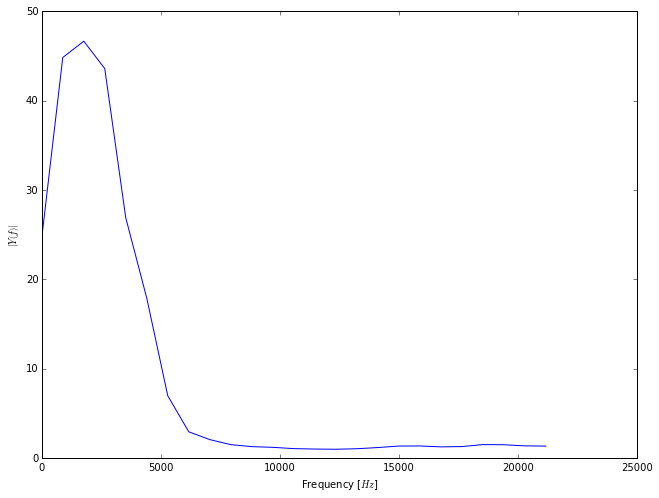
\includegraphics[width=\textwidth]{Links.png}
    	\caption{Links}
        \label{fig:Links}
    \end{subfigure}
    ~
    \begin{subfigure}[b]{0.49\textwidth}        		   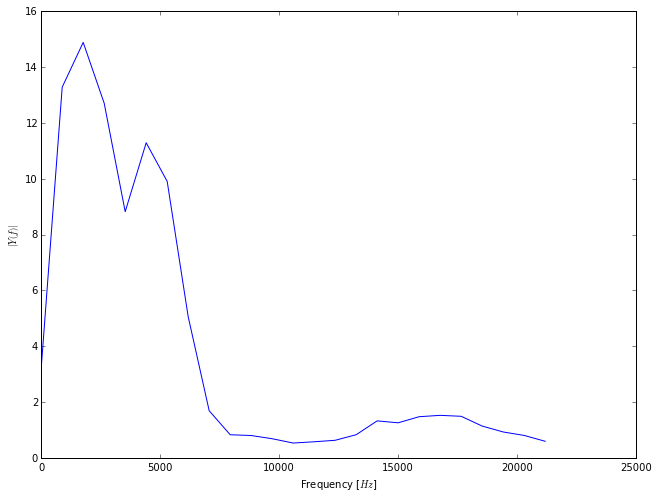
\includegraphics[width=\textwidth]{Rechts.png}
       \caption{Rechts}
       \label{fig:Rechts}
    \end{subfigure}
\caption{Referenzspektren der einzelnen Wörter}
\label{fig:RefSpektren}
\end{figure}

\begin{figure}[H]
\centering
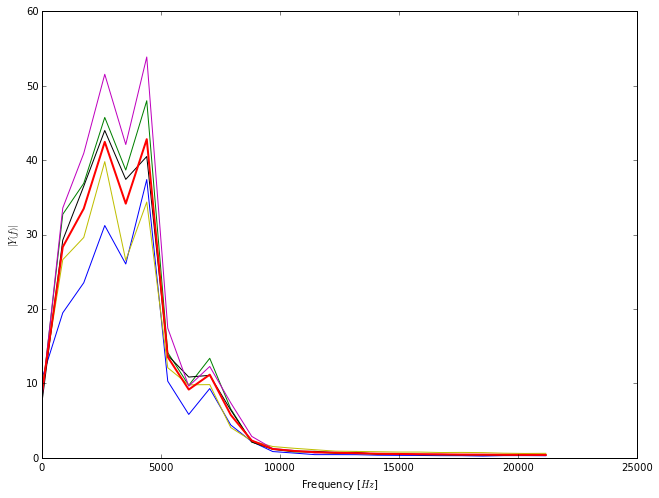
\includegraphics[width=0.75\textwidth]{vergleich.png}
\caption{Mittelwert eines Referenzspektrums mit einzelnen Spektren}
\label{fig:MittelwertSpek}
\end{figure}


\section{Auswertung und Interpretation}
\label{chap:AUSWERTUNGUNDINTERPRETATION}
In Abbildung \ref{fig:RefSpektren} sind die Referenzspektren zu den einzelnen Worten zu sehen. Auf der X-Achse ist die Frequenz aufgetragen und auf der Y-Achse die Amplitude.
Die Frequenzen mit den höchsten Amplituden halten sich in einem Bereich von 0 - $\approx 10 kHz$ auf. Dieses Ergebnis passt in das Frequenzband der Menschlichen Stimme hinein. \cite{WikiMensch} Bei den Wörtern Rechts und Links scheinen mit die Größten Frequenzen vorhanden zu sein. Diese übersteigen das Frequenzband der menschlichen Stimme und werden daher auf den Zischlaut s zurückgeführt, der in beiden Worten Links bzw. Rechts vorhanden ist. 
Abbildung \ref{fig:MittelwertSpek} sind die Spektren der einzelnen Messungen für das Wort 'Hoch', verschiedenfarbig zu sehen. Die etwas dickere rote Linie ist der Mittelwert über alle aufgenommenen Spektren des Signals und wird als Referenzspektrum für das Wort Hoch benutzt. Es zeichnet sich eine Charakteristik für das Wort 'Hoch' ab, welche sich im Mittelwert widerspiegelt.

Insgesamt wurden 34 von 40 Wörtern richtig erkannt. Prozentual bedeutet das, dass der Spracherkenner eine Trefferquote von 85\% hat. Bei den Testaufnahmen des Referenzsprechers gab es eine Trefferquote von 100\%. Die Aufnahmen des anderen Sprechers wurden zu 70\% korrekt erkannt. Sechs von Zwanzig Aufnahmen sind von diesem Testdatensatz nicht korrekt erkannt worden. Dieses Ergebnis ist erfreulich. Es entspricht den Erwartungen, dass der Testdatensatz des Sprechers, der auch die Referenzaufnahmen gesprochen hat besser korellieren, da der Spracherkenner quasi auf seine Stimme getrimmt wurde. Nicht jeder Mensch hat die gleiche Stimmtonlage, deshalb wurden auch weniger Wörter des zweiten Testsprechers erkannt. Allerdings sind mehr als die Hälfte der Wörter, welche der Sprecher B sprach erkannt wurden. Auch dies ist ein positives Resultat. Der Spracherkenner scheint somit gelungen zu sein.


